% Emacs, this is -*-latex-*-

\ex{Mean field variational inference I}
\label{ex:MFVI-I}
Let $\ELBOx(q)$ be the evidence lower bound for the marginal $p(\x)$ of a joint pdf/pmf $p(\x,\y)$,
\begin{equation}
  \ELBOx(q) = \E_{q(\y|\x)} \left[\log \frac{p(\x,\y)}{q(\y|\x)}\right].
  \end{equation}
Mean field variational inference assumes that the variational distribution $q(\y|\x)$ fully factorises, i.e.
\begin{equation}
  q(\y | \x) = \prod_{i=1}^d q_i(y_i | \x),
\end{equation}
when $\y$ is $d$-dimensional. An approach to learning the $q_i$ for
each dimension is to update one at a time while keeping the others fixed. We
here derive the corresponding update equations.

\begin{exenumerate}
\item Show that the evidence lower bound $\ELBOx(q)$ can be written as
\begin{equation}
  \ELBOx(q) = \E_{q_1(y_1|\x)} \E_{q(\y_{\setminus 1}|\x)}\left[ \log p(\x,\y)\right] - \sum_{i=1}^d \E_{q_i(y_i|\x)} \left[\log q_i(y_i|\x)\right]
\end{equation}
where $q(\y_{\setminus 1}|\x) = \prod_{i=2}^d q_i(y_i | \x)$ is the variational distribution without $q_1(y_1|\x)$.

\begin{solution}
  This follows directly from the definition of the ELBO and the assumed factorisation of $q(\y|\x)$. We have
  \begin{align}
    \ELBOx(q) &= \E_{q(\y|\x)} \log p(\x,\y) - \E_{q(\y|\x)} \log q(\y|\x) \\
    & = \E_{ \prod_{i=1}^d q_i(y_i | \x)}  \log p(\x,\y) - \E_{ \prod_{i=1}^d q_i(y_i | \x)} \sum_{i=1}^d \log q_i(y_i|\x) \\
    & = \E_{ \prod_{i=1}^d q_i(y_i | \x)}  \log p(\x,\y) - \sum_{i=1}^d  \E_{q_i(y_i | \x)} \log q_i(y_i|\x) \\
    & = \E_{q_1(y_1|\x)} \E_{ \prod_{i=2}^d q_i(y_i | \x)}  \log p(\x,\y) - \sum_{i=1}^d  \E_{q_i(y_i | \x)} \log q_i(y_i|\x)\\
    & = \E_{q_1(y_1|\x)} \E_{q(\y_{\setminus 1}|\x)}\left[ \log p(\x,\y)\right] - \sum_{i=1}^d \E_{q_i(y_i|\x)} \left[\log q_i(y_i|\x)\right]
  \end{align}
  We have here used the linearity of expectation. In case of continuous random variables, for instance, we have
  \begin{align}
 \E_{ \prod_{i=1}^d q_i(y_i | \x)} \sum_{i=1}^d \log q_i(y_i|\x) & = \int  q_1(y_1 | \x)\cdot \ldots\cdot q_d(y_d|\x)  \sum_{i=1}^d \log q_i(y_i|\x) d y_1\ldots d y_d\\
 & =  \sum_{i=1}^d \int q_1(y_1 | \x)\cdot \ldots \cdot q_d(y_d|\x) \log q_i(y_i|\x) d y_1\ldots d y_d\\
 & =  \sum_{i=1}^d \int q_i(y_i | \x)\log q_i(y_i|\x) d y_i \underbrace{\int \prod_{j\neq i} q_j(y_j|\x) d y_j}_{=1}\\
 & =  \sum_{i=1}^d E_{q_i(y_i|\x)} \log q_i(y_i|\x)
\end{align}
For discrete random variables, the integral is replaced with a sum and leads to the same result.

\end{solution}

\item Assume that we would like to update $q_1(y_1 |\x)$ and that the
  variational marginals of the other dimensions are kept fixed. Show that
  \begin{equation}
    \argmax_{q_1(y_1|\x)} \ELBOx(q) = \argmin_{q_1(y_1|\x)} \KL(q_1(y_1|\x) || \bar{p}(y_1|\x))
  \end{equation}
  with
\begin{equation}
  \log \bar{p}(y_1|\x) = \E_{q(\y_{\setminus 1}|\x)}\left[ \log p(\x,\y)\right] + \text{const},
\end{equation}
where $\text{const}$ refers to terms not depending on $y_1$. That is,
\begin{equation}
\bar{p}(y_1|\x) = \frac{1}{Z} \exp\left[ \E_{q(\y_{\setminus
      1}|\x)}\left[ \log p(\x,\y)\right] \right],
\end{equation}
where $Z$ is the normalising constant. Note that variables $y_2, \ldots, y_d$
are marginalised out due to the expectation with respect to $q(\y_{\setminus
  1}|\x)$.

  \begin{solution}
    Starting from 
    \begin{equation}
      \ELBOx(q) = \E_{q_1(y_1|\x)} \E_{q(\y_{\setminus 1}|\x)}\left[ \log p(\x,\y)\right] - \sum_{i=1}^d \E_{q_i(y_i|\x)} \left[\log q_i(y_i|\x)\right]
    \end{equation}
    we drop terms that do not depend on $q_1$. We then obtain
    \begin{align}
      J(q_1) & =  \E_{q_1(y_1|\x)} \E_{q(\y_{\setminus 1}|\x)}\left[ \log p(\x,\y)\right] -  \E_{q_1(y_1|\x)} \left[\log q_1(y_1|\x)\right]\\
      & = \E_{q_1(y_1|\x)} \log \bar{p}(y_1|\x) - \E_{q_1(y_1|\x)} \left[\log q_1(y_1|\x)\right] + \text{const}\\
      & = \E_{q_1(y_1|\x)}\left[ \log \frac{\bar{p}(y_1|\x)}{ q_1(y_1|\x)} \right]\\
      & = -\KL( q_1(y_1|\x) || \bar{p}(y_1|\x) )
    \end{align}
    Hence
    \begin{equation}
      \argmax_{q_1(y_1|\x)} \ELBOx(q) = \argmin_{q_1(y_1|\x)} \KL(q_1(y_1|\x) || \bar{p}(y_1|\x))
    \end{equation}
    
  \end{solution}

\item Conclude that given $q_i(y_i|\x)$, $i=2, \ldots, d$, the optimal $q_1(y_1|\x)$ equals $\bar{p}(y_1|\x)$.

  This then leads to an iterative updating scheme where we cycle
  through the different dimensions, each time updating the corresponding marginal variational distribution according to:
  \begin{align}
    q_i(y_i|\x) &=  \bar{p}(y_i|\x), &  \bar{p}(y_i|\x) &= \frac{1}{Z} \exp\left[ \E_{q(\y_{\setminus i}|\x)}\left[ \log p(\x,\y)\right] \right]
  \end{align}
  where $q(\y_{\setminus i}|\x) = \prod_{j \neq i} q(y_j | \x)$ is the product of all marginals without marginal $q_i(y_i|\x)$.

  \begin{solution}
    This follows immediately from the fact that the KL divergence is
    minimised when $q_1(y_1|\x) = \bar{p}(y_1|\x)$. Side-note: The
    iterative update rule can be considered to be coordinate ascent
    optimisation in function space, where each ``coordinate''
    corresponds to a $q_i(y_i|\x)$.
    
  \end{solution}
\end{exenumerate}

% --------------------------------------------------

\ex{Mean field variational inference II}
Assume random variables $y_1, y_2, x$ are generated according to the following process
\begin{align}
  y_1 &\sim \Gauss(y_1; 0, 1) &   y_2 &\sim \Gauss(y_2; 0, 1) \\
  n &\sim \Gauss(n; 0, 1)    &    x & = y_1+y_2+n & 
\end{align}
where $y_1, y_2, n$ are statistically independent.

\begin{exenumerate}

\item $y_1, y_2, x$ are jointly Gaussian. Determine their mean and their
  covariance matrix.

  \begin{solution}
    
    The expected value of $y_1$ and $y_2$ is zero. By linearity of
    expectation, the expected value of $x$ is
    \begin{equation}
      \E(x) = \E(y_1) + \E(y_2) + \E(n) = 0
    \end{equation}
    The variance of $y_1$ and $y_2$ is 1. Since $y_1, y_2, n$ are statistically independent,
    \begin{equation}
      \Var(x) = \Var(y_1) + \Var(y_2) + \Var(n) = 1 + 1 + 1 = 3.
    \end{equation}
    The covariance between $y_1$ and $x$ is
    \begin{align}
      \text{cov}(y_1, x) &= \E( (y_1-\E(y_1))(x-\E(x))) = \E( y_1 x) \\
      &= \E( y_1(y_1+y_2+n) ) = \E(y_1^2) + \E(y_1 y_2) + \E(y_1 n)\\
      &= 1 +  \E(y_1)\E(y_2) + \E(y_1)\E(n)\\
      &= 1 + 0 + 0
    \end{align}
    where we have used that $y_1$ and $x$ have zero mean and the independence assumptions.

    The covariance between $y_2$ and $x$ is computed in the same way and equals 1 too.

    We thus obtain the covariance matrix $\Sigmab$,
    \begin{equation}
      \Sigmab = \begin{pmatrix}
        1 & 0 & 1\\
        0 & 1 & 1\\
        1 & 1 & 3
      \end{pmatrix}
    \end{equation}
    
  \end{solution}

\item The conditional $p(y_1, y_2 | x)$ is Gaussian with mean $\m$ and covariance $\C$,
  \begin{align}
    \m &= \frac{x}{3} \begin{pmatrix}
      1\\
      1
    \end{pmatrix}
    &
    \C & = \frac{1}{3} \begin{pmatrix}
      2 &-1 \\
     -1 & 2
    \end{pmatrix}
  \end{align}
  Since $x$ is the sum of three random variables that have the
  same distribution, it makes intuitive sense that the mean assigns
  $1/3$ of the observed value of $x$ to $y_1$ and $y_2$. Moreover,
  $y_1$ and $y_2$ are negatively corrected since an increase in $y_1$
  must be compensated with a decrease in $y_2$.

  Let us now approximate the posterior $p(y_1, y_2 | x)$ with mean
  field variational inference. Determine the optimal variational
  distribution using the method and results from \exref{ex:MFVI-I}. You may use that
  \begin{align}
    p(y_1, y_2, x) &= \Gauss\left( (y_1, y_2, x); \zerob, \Sigmab \right) &  \Sigmab &= \begin{pmatrix} 
      1 & 0 & 1\\
      0 & 1 & 1\\
      0 & 1 & 3
    \end{pmatrix}
    &
    \Sigmab^{-1} &= \begin{pmatrix} 
      2 & 1 & -1\\
      1 & 2 & -1\\
      -1 & -1 & 1
    \end{pmatrix}
  \end{align}
  
  \begin{solution}
    The mean field assumption means that the variational distribution is assumed to factorise as
    \begin{equation}
      q(y_1, y_2 | x) = q_1(y_1 | x) q_2(y_2 | x)
    \end{equation}
    From \exref{ex:MFVI-I}, the optimal $q_1(y_1|x)$ and $q_2(y_2|x)$ satisfy
     \begin{align}
       q_1(y_1|x) &=  \bar{p}(y_1|x), &  \bar{p}(y_1|x) &= \frac{1}{Z} \exp\left[ \E_{q_2(y_2|x)}\left[ \log p(y_1, y_2, x)\right] \right]\\
       q_2(y_2|x) &=  \bar{p}(y_2|x), &  \bar{p}(y_2|x) &= \frac{1}{Z} \exp\left[ \E_{q_1(y_1|x)}\left[ \log p(y_1, y_2, x)\right] \right]
     \end{align}
    Note that these are coupled equations: $q_2$ features in the
    equation for $q_1$ via $\bar{p}(y_1|x)$, and $q_1$ features in
    the equation for $q_2$ via $\bar{p}(y_2|x)$. But we have two
    equations for two unknowns, which for the Gaussian joint model
    $p(x, y_1, y_2)$ can be solved in closed form.

    Given the provided equation for $p(y_1, y_2, x)$, we have that
    \begin{align}
      \log p(y_1, y_2, x) & = -\frac{1}{2} \begin{pmatrix}
        y_1\\
        y_2\\
        x
      \end{pmatrix}^\top
      \begin{pmatrix}
        2 & 1 & -1\\
        1 & 2 & -1\\
        -1 & -1 & 1
      \end{pmatrix}
      \begin{pmatrix}
        y_1\\
        y_2\\
        x
      \end{pmatrix} + \text{const}\\
        & = -\frac{1}{2} \left( 2 y_1^2 + 2 y_2^2 + x^2 + 2 y_1 y_2 - 2 y_1 x - 2y_2 x \right) + \text{const}
    \end{align}
    
    Let us start with the equation for $\bar{p}(y_1|x)$. It is easier to work in the logarithmic domain, where we obtain:
    \begin{align}
      \log  \bar{p}(y_1|x) & =  \E_{q_2(y_2|x)}\left[ \log p(y_1, y_2, x)\right] + \text{const}\\
      & = -\frac{1}{2} \E_{q_2(y_2|x)}\left[  2 y_1^2 + 2 y_2^2 + x^2 + 2 y_1 y_2 - 2 y_1 x - 2y_2 x \right] + \text{const}\\
      & = -\frac{1}{2} \left(2 y_1^2 + 2 y_1 \E_{q_2(y_2|x)}[y_2] - 2 y_1 x \right) + \text{const}\\
      & = -\frac{1}{2} \left( 2 y_1^2 +2y_1 m_2 - 2 y_1 x \right) + \text{const}\\
      & = -\frac{1}{2} \left( 2 y_1^2 - 2 y_1 (x-m_2) \right) + \text{const}
      \label{eq:barp1}
    \end{align}
    where we have absorbed all terms not involving $y_1$ into the constant. Moreover, we set $\E_{q_2(y_2|x)}[y_2]=m_2$.

    Note that an arbitrary Gaussian density $\Gauss(y; m, \sigma^2)$
    with mean $m$ and variance $\sigma^2$ can be written in the
    log-domain as
    \begin{align}
      \log \Gauss(y; m, \sigma^2) & = -\frac{1}{2}\frac{(y-m)^2}{\sigma^2} + \text{const}\\
      & = -\frac{1}{2} \left( \frac{y^2}{\sigma^2} -2y \frac{m}{\sigma^2} \right) + \text{const}
      \label{eq:loggauss}
    \end{align}
    Comparison with \eqref{eq:barp1} shows that $\bar{p}(y_1|x)$, and
    hence $q_1(y_1 | x)$, is Gaussian with variance and mean equal to
    \begin{align}
      \sigma_1^2 &= \frac{1}{2} & m_1 & = \frac{1}{2}(x-m_2)
    \end{align}
    Note that we have not made a Gaussianity assumption on $q_1(y_1 |
    x)$. The optimal $q_1(y_1 | x)$ turns out to be Gaussian because
    the model $p(y_1, y_2, x)$ is Gaussian.
    
    The equation for $\bar{p}(y_2|x)$ gives similarly
    \begin{align}
      \log  \bar{p}(y_2|x) & =  \E_{q_1(y_1|x)}\left[ \log p(y_1, y_2, x)\right] + \text{const}\\
      & = -\frac{1}{2} \E_{q_1(y_1|x)}\left[  2 y_1^2 + 2 y_2^2 + x^2 + 2 y_1 y_2 - 2 y_1 x - 2y_2 x \right] + \text{const}\\
      & = -\frac{1}{2} \left(2 y_2^2 + 2 \E_{q_1(y_1|x)}[y_1] y_2 - 2y_2 x \right) + \text{const}\\
      & = -\frac{1}{2} \left(2 y_2^2 + 2 m_1 y_2 - 2 y_2 x \right) + \text{const}\\
      & = -\frac{1}{2} \left(2 y_2^2 - 2 y_2(x-m_1) \right) + \text{const}
      \label{eq:barp2}
    \end{align}
    where we have absorbed all terms not involving $y_2$ into the
    constant. Moreover, we set $\E_{q_1(y_1|x)}[y_1]=m_1$. With
    \eqref{eq:loggauss}, this is defines a Gaussian distribution with 
    variance and mean equal to
    \begin{align}
      \sigma_2^2 &= \frac{1}{2} & m_2 & = \frac{1}{2}(x-m_1)
    \end{align}
    Hence the optimal marginal variational distributions $q_1(y_1|x)$ and
    $q_2(y_2|x)$ are both Gaussian with variance equal to $1/2$. Their
    means satisfy
    \begin{align}
      m_1 & = \frac{1}{2}(x-m_2) & m_2  & = \frac{1}{2}(x-m_1)
    \end{align}
    These are two equations for two unknowns. We can solve them as follows   
    \begin{align}
      2 m_1 &= x - m_2 \\
      & = x -\frac{1}{2}(x-m_1)\\
      4 m_1 & = 2 x -x + m_1 \\
      3 m_1 & = x\\
      m_1 & = \frac{1}{3} x
    \end{align}
    Hence
    \begin{equation}
     m_2 = \frac{1}{2} x - \frac{1}{6} x = \frac{2}{6} x = \frac{1}{3} x
    \end{equation}
    In summary, we find
    \begin{align}
      q_1(y_1 | x) & = \Gauss\left(y_1; \frac{x}{3}, \frac{1}{2}\right) &  q_2(y_2 | x) & = \Gauss\left(y_2; \frac{x}{3}, \frac{1}{2}\right)
    \end{align}
    and the optimal variational distribution $q(y_1, y_2|x) =
    q_1(y_1|x) q_2(y_2|x)$ is Gaussian. We have made the mean field
    (independence) assumption but not the Gaussianity
    assumption. Gaussianity of the variational distribution is a
    consequence of the Gaussianity of the model $p(y_1, y_2, x)$.

    Comparison with the true posterior shows that the mean field
    variational distribution $q(y_1, y_2 | x)$ has the same mean but
    ignores the correlation and underestimates the marginal
    variances. The true posterior and the mean field approximation are
    shown in Figure \ref{fig:meanfield}.

    \begin{figure}[h!]
      \centering
      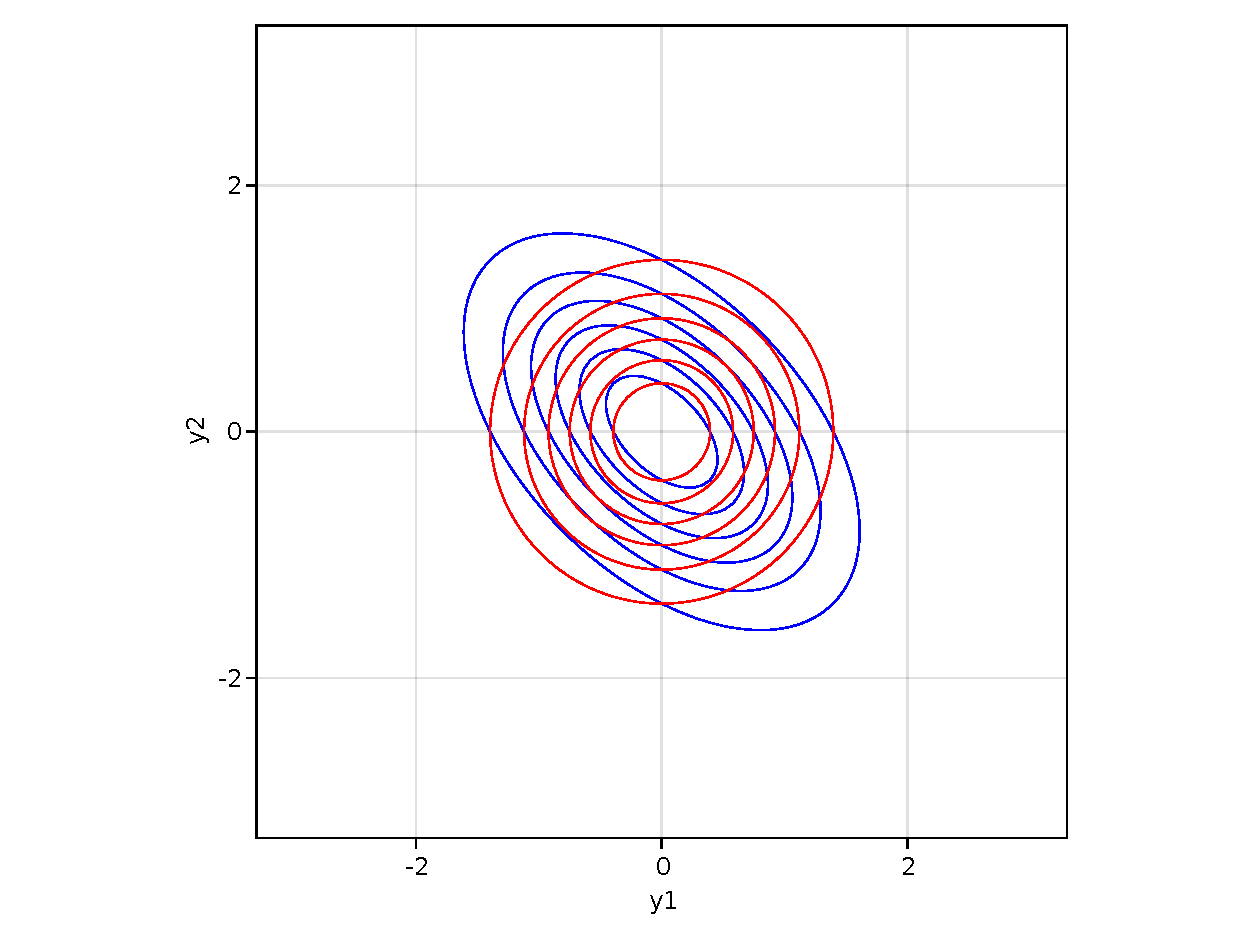
\includegraphics[width=0.75\textwidth]{meanfield}
      \caption{\label{fig:meanfield}In blue: correlated true posterior. In red: mean field approximation.}
    \end{figure}
  \end{solution}


  
\end{exenumerate}
% --------------------------------------------------
\ex{Variational posterior approximation I}

We have seen that maximising the evidence lower bound (ELBO) with
respect to the variational distribution $q$ minimises the
Kullback-Leibler divergence to the true posterior $p$. We here assume
that $q$ and $p$ are probability density functions so that the
Kullback-Leibler divergence between them is defined as
\begin{equation}
  \KL(q || p) = \int q(\x) \log \frac{q(\x)}{p(\x)} \ud \x = \E_q \left[\log \frac{q(\x)}{p(\x)}\right].
\end{equation}


\begin{exenumerate}

\item You can here assume that $\x$ is one-dimensional so that $p$
  and $q$ are univariate densities. Consider the case where $p$ is
  a bimodal density but the variational densities $q$ are
  unimodal. Sketch a figure that shows $p$ and a variational
  distribution $q$ that has been learned by minimising $\text{KL}(q
  || p)$. Explain qualitatively why the sketched $q$ minimises
  $\text{KL}(q || p)$.

  \begin{solution}

  A possible sketch is shown in the figure below.

  \begin{figure}[h!]
    \centering
    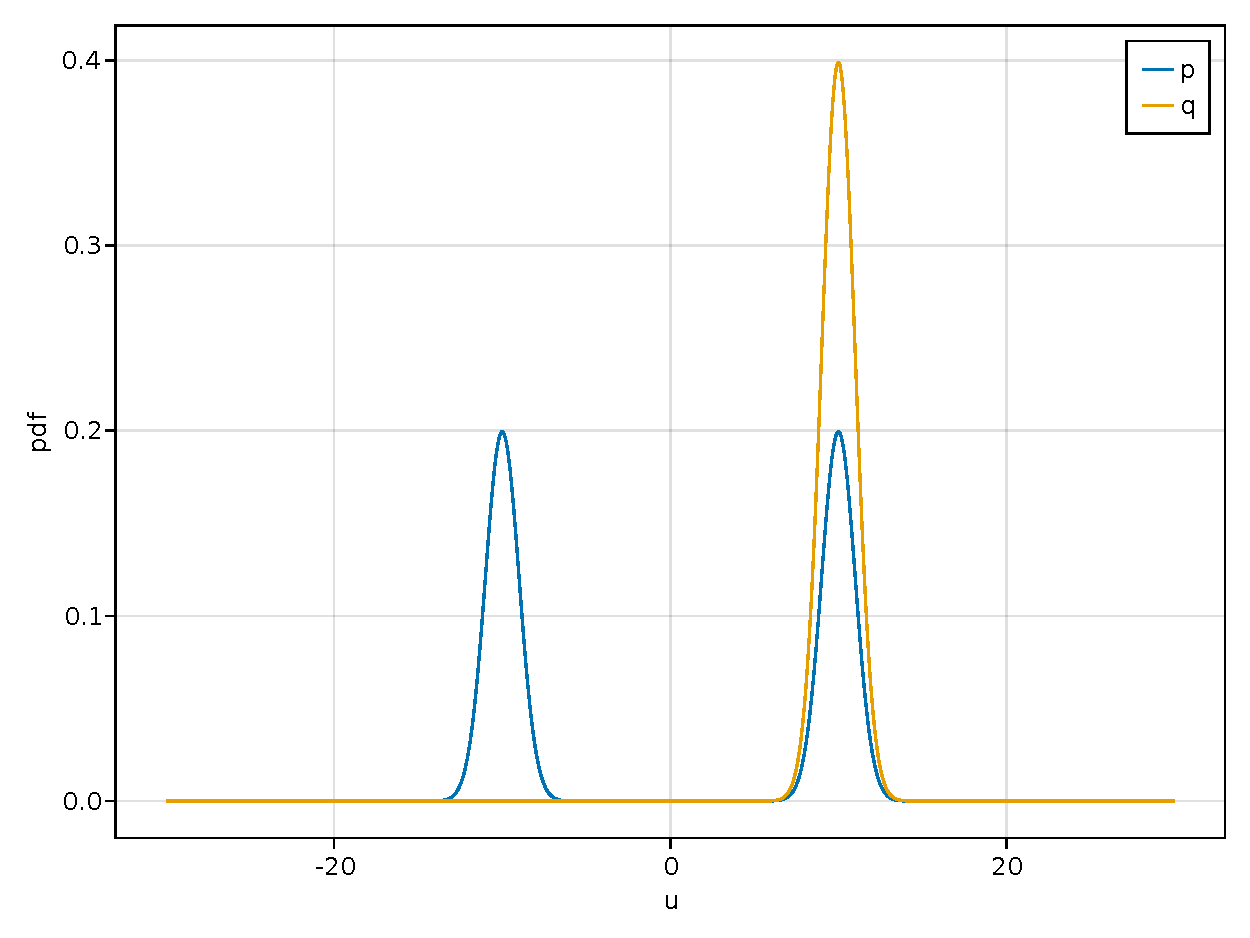
\includegraphics[width = 0.5 \textwidth]{KL-asym}
  \end{figure}

  Explanation: We can divide the domain of $p$ and $q$ into the areas
  where $p$ is small (zero) and those where $p$ has significant
  mass. Since the objective features $q$ in the numerator while $p$ is
  in the denominator, an optimal $q$ needs to be zero where $p$ is
  zero. Otherwise, it would incur a large penalty (division by
  zero). Since we take the expectation with respect to $q$, however,
  regions where $p>0$ do not need to be covered by $q$; cutting them
  out does not incur a penalty. Hence, optimal unimodal $q$ only cover
  one peak of the bimodal $p$.
   
  \end{solution}

  
\item Assume that the true posterior $p(\x) = p(x_1, x_2)$ factorises into two Gaussians of mean zero and variances $\sigma_1^2$ and $\sigma_2^2$,
  \begin{equation}
    p(x_1,x_2) = \frac{1}{\sqrt{2\pi \sigma_1^2}} \exp\left[-\frac{x_1^2}{2 \sigma_1^2}\right]\frac{1}{\sqrt{2\pi \sigma_2^2}} \exp\left[-\frac{x_2^2}{2 \sigma_2^2}\right].
  \end{equation}
  Assume further that the variational density $q(x_1,x_2; \lambda^2)$ is parametrised as
  \begin{equation}
    q(x_1,x_2;\lambda^2) = \frac{1}{2\pi \lambda^2} \exp\left[-\frac{x_1^2+x_2^2}{2 \lambda^2}\right]
    \end{equation}
  where $\lambda^2$ is the variational parameter that is learned
  by minimising $ \KL(q || p)$. If $\sigma^2_2$ is much
  larger than $\sigma^2_1$, do you expect $\lambda^2$ to be closer to $\sigma_2^2$
  or to $\sigma_1^2$? Provide an explanation.

  \begin{solution}
    The learned variational parameter will be closer to $\sigma_1^2$
    (the smaller of the two $\sigma_i^2$).
      
    Explanation: First note that the $\sigma_i^2$ are the variances
    along the two different axes, and that $\lambda^2$ is the single
    variance for both $x_1$ and $x_2$. The objective penalises $q$ if
    it is non-zero where $p$ is zero (see above). The variational
    parameter $\lambda^2$ thus will get adjusted during learning so
    that the variance of $q$ is close to the smallest of the two
    $\sigma_i^2$.

  \end{solution}

\end{exenumerate}

% --------------------------------------------------

\ex{Variational posterior approximation II}

We have seen that maximising the evidence lower bound (ELBO) with
respect to the variational distribution minimises the
Kullback-Leibler divergence to the true posterior. We here
investigate the nature of the approximation if the family of
variational distributions does not include the true posterior.

\begin{exenumerate}

\item Assume that the true posterior for $\x = (x_1, x_2)$ is given by
  \begin{equation}
    p(\x) = \normal(x_1 ; \sigma_1^2)\normal(x_2 ; \sigma_2^2) 
  \end{equation}
  and that our variational distribution $q(\x; \lambda^2)$ is
  \begin{equation}
    q(\x; \lambda^2) = \normal(x_1 ; \lambda^2)\normal(x_2 ; \lambda^2),
  \end{equation}
  where $\lambda >0$ is the variational parameter. Provide an
  equation for
  \begin{equation}
    J(\lambda) = \KL(q(\x; \lambda^2) || p(\x)),
  \end{equation}
  where you can omit additive terms that do not depend on
  $\lambda$. 

  \begin{solution}

    We write
    \begin{align}
      \text{KL}(q(\x; \lambda^2) || p(\x)) & = \E_q \left[ \log  \frac{q(\x; \lambda^2)}{p(\x)} \right]\\
      & = \E_q \log q(\x; \lambda^2) - \E_q \log p(\x)\\
      & = \E_q \log  \normal(x_1 ; \lambda^2) + \E_q \log \normal(x_2 ; \lambda^2) \nonumber \\
      & \phantom{=} - \E_q \log \normal(x_1 ; \sigma_1^2) - \E_q \log \normal(x_2 ; \sigma_2^2)
    \end{align}
    
    We further have
    \begin{align}
      \E_q \log  \normal(x_i ; \lambda^2) & = \E_q \log \left[ \frac{1}{\sqrt{2\pi \lambda^2}} \exp \left[-\frac{x_i^2}{2 \lambda^2} \right] \right]\\
      & = \log \left[ \frac{1}{\sqrt{2\pi \lambda^2}}\right] -\E_q \left[\frac{x_i^2}{2 \lambda^2}\right]\\
      & = -\log \lambda - \frac{\lambda^2}{2\lambda^2} + \text{const}\\
      & = -\log \lambda - \frac{1}{2} + \text{const}\\
      & = -\log \lambda + \text{const}
    \end{align}
    where we have used that for zero mean $x_i$, $\E_q [x_i^2] = \var(x_i) = \lambda^2$. 

    We similarly obtain
    \begin{align}
    \E_q \log \normal(x_i ; \sigma_i^2) & = \E_q \log \left[ \frac{1}{\sqrt{2\pi \sigma_i^2}} \exp \left[-\frac{x_i^2}{2 \sigma_i^2} \right] \right]\\
      & = -\log \left[ \frac{1}{\sqrt{2\pi \sigma_i^2}}\right] -\E_q \left[\frac{x_i^2}{2 \sigma_i^2}\right]\\
    & = -\log \sigma_i - \frac{\lambda^2}{2\sigma_i^2} + \text{const}\\
    & = - \frac{\lambda^2}{2\sigma_i^2} + \text{const}
    \end{align}
    
    We thus have
    \begin{align}
      \text{KL}(q(\x; \lambda^2 || p(\x))  & =  -2 \log \lambda + \lambda^2\left(\frac{1}{2\sigma_1^2}+\frac{1}{2\sigma_2^2}\right)+\text{const}
    \end{align}    
    
  \end{solution}


  
\item Determine the value of $\lambda$ that minimises $J(\lambda) =
  \KL(q(\x; \lambda^2) || p(\x))$. Interpret the result and
  relate it to properties of the Kullback-Leibler
  divergence.

  \begin{solution}

    Taking derivatives of $J(\lambda)$ with respect to $\lambda$ gives
    \begin{align}
      \frac{\partial J(\lambda)}{\partial \lambda} & = -\frac{2}{\lambda} + \lambda \left(\frac{1}{\sigma_1^2}+\frac{1}{\sigma_2^2}\right)
      \end{align}
    Setting it zero yields
    \begin{align}
      \frac{1}{\lambda^2} &= \frac{1}{2}\left(\frac{1}{\sigma_1^2}+\frac{1}{\sigma_2^2}\right)
    \end{align}
    so that
    \begin{align}
      \lambda^2 = 2 \frac{\sigma_1^2 \sigma_2^2}{\sigma_1^2+\sigma_2^2}
    \end{align}
    or
    \begin{equation}
    \lambda = \sqrt{2} \sqrt{\frac{\sigma_1^2 \sigma_2^2}{\sigma_1^2+\sigma_2^2}}
    \end{equation}
    This is a minimum because the second derivative of
    $J(\lambda)$
    \begin{equation}
      \frac{\partial^2 J(\lambda)}{\partial \lambda^2} = \frac{2}{\lambda^2} + \left(\frac{1}{\sigma_1^2}+\frac{1}{\sigma_2^2}\right)
    \end{equation}
    is positive for all $\lambda > 0$.
    
    The result has an intuitive explanation: the optimal variance
    $\lambda^2$ is the harmonic mean of the variances $\sigma_i^2$ of
    the true posterior. In other words, the optimal precision
    $1/\lambda^2$ is given by the average of the precisions
    $1/\sigma_i^2$ of the two dimensions.

    If the variances are not equal, e.g.\ if $\sigma_2^2 >
    \sigma_1^2$, we see that the optimal variance of the variational
    distribution strikes a compromise between two types of penalties
    in the KL-divergence: the penalty of having a bad fit because the
    variational distribution along dimension two is too narrow; and
    along dimension one, the penalty for the variational distribution
    to be nonzero when $p$ is small. 

  \end{solution}
  
\end{exenumerate}

